% Created 2021-12-29 Wed 05:01
% Intended LaTeX compiler: pdflatex
\documentclass[11pt]{article}
\usepackage[utf8]{inputenc}
\usepackage[T1]{fontenc}
\usepackage{graphicx}
\usepackage{longtable}
\usepackage{wrapfig}
\usepackage{rotating}
\usepackage[normalem]{ulem}
\usepackage{amsmath}
\usepackage{amssymb}
\usepackage{capt-of}
\usepackage{hyperref}
\author{Ian Gomez}
\date{\today}
\title{Efficient PAC Learning from the crowd}
\hypersetup{
 pdfauthor={Ian Gomez},
 pdftitle={Efficient PAC Learning from the crowd},
 pdfkeywords={},
 pdfsubject={},
 pdfcreator={Emacs 27.1 (Org mode 9.6)}, 
 pdflang={English}}
\begin{document}

\maketitle
\tableofcontents

notes were made after I read the Intro and notation however the core idea is that we want to create an algorithm to efficiently learn from a crowd of generated data where we cannot assure how correct a label is from a given labeler, and we want to do this with low label cost, and high accuracy.
The main idea is to use boosting methods and interleave the data collection process with the boosting algorithm since most papers focused on data collection and learning from noisy data as seperate tasks. this paper novelly interleaves both to make an algorithm which has better performance.
\section{3. A baseline algorithm}
\label{sec:orga4b3fbb}
\begin{itemize}
\item The baseline algorithm is simple in that we query k workers and take the majority vote from those k workers for each sample in the dataset.
\item The main problem is that the amount of workers needed to statistically guarentee all labels are correct scales in \(O(log(m/\delta))\)
\item Second when the number of perfect labelers < 1/2 there can be errors in the dataset which means the final classifier will have bad performance
\item To solve this we mix probablistic filtering and boosting algorithms to solve the problems mentioned prior
\item This also provides a good way of finding perfect labelers in the sense that we can query labelers on a test set of images and iteratively discard labelers who get a label wrong.
\end{itemize}
\section{4. An Interleaving Algorithm.}
\label{sec:orgcbc8cd5}
\begin{itemize}
\item For this we utilize research done by Schapire on boosting algorithms. Specifically we use the fact that with 3 classifiers you can achieve O(p\textsuperscript{2}) error with classifiers that get error p = 0.5 - y where y is small.
\item Schapire proved that with 3 classifers h1, h2, h3 where \(err_D(h_1) \leq p\), \(err_{D2}(h2) \leq p\), \(err_{D3}(h3) \leq p\) that \(err_D(Maj(h_1,h_2,h_3)) \leq O(p^2)\)
\item As opposed to the originally learning p = 0.5 - y we extend this to any p where we sample \(m_{p,\delta}\). Where as p increases the label cost decreases.
\item We particularly use this to learn classifier \(h_1\) of \(O(\sqrt{\epsilon)}\) using \(O(m_{\sqrt{\epsilon},\delta})\) that are labeled with \(O(log(m_{\sqrt{\epsilon},\delta}))\)
\item Given classifier \(h_1\) which is trained on dataset D. we construct \(D_2\) such that \(D_2 = \frac{1}{2} D_I + \frac{1}{2} D_C\)
\item The reasoning is that we want to get informative samples which \(h_1\) will perform poorly on.
\item However, when constructing \(D_2\) it becomes difficult to construct a dataset such that half of the samples incorrect since it will only be incorrect with probability P.
\item Therefore we must construct a faster filtering algorithm.
\item Filter algorithm
\item The idea is that we gather \(N=log(\frac{1}{\epsilon})\) workers and for each sample we compute the majority of \(L_1 ... L_k\) such that k is odd. if \(Maj(L_1...L_k) = h_1(x)\) then stop for that sample.
\item If we manage to iterate through all N then we add the sample to \(D_I\)
\item This algorithm makes it so that \(D_I\) is found with constant overhead to the original label complexity
\item due to the fact that eventually the majority will equal the classifier prediction given some classification accuracy > 0.5 for all correctly labeled samples.
\item Lemma 4.9 proves that this happens with a constant time in most cases.
\item For the case where we find incorrectly labeled samples it is very unlikely that the labeler gets it wrong since the probability that the majority is incorrect is small
\item Because the probability of being wrong is 1-p therefore the probability that the majority over all iterations is wrong is very small.
\item This is proved in Lemma 4.6
\item In essence we are super sampling with the filter algorithm. The idea is that when in the realizable setting we can super sample from \(D_2\) such that we can construct a new distribution which is a constant density higher than that of the original \(D_2\). It is proven that this super sampled dataset performs with a constant performance.
\item We then arrive at this algorithm.
\end{itemize}
\begin{center}
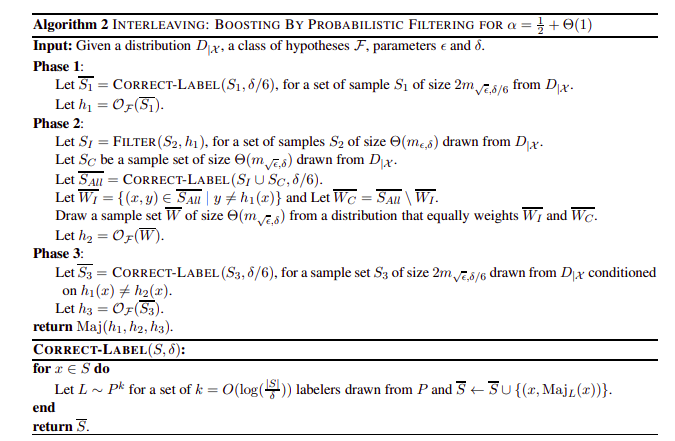
\includegraphics[width=.9\linewidth]{./images/Algo2.png}
\end{center}
\begin{itemize}
\item which has \(\Lambda = O(\sqrt{\epsilon}log(\frac{m_{\sqrt{\epsilon},\delta}}{\delta})+1)\) label cost. where this is constant if \(1/\sqrt{\epsilon} \geq log(...)\)
\item Insert lots of proofs on why this works.
\item First proof is on why Filter behaves well
\item Second proof is on why \(err(h_2) = O(\sqrt{e})\)
\item Third proof is on why filter only has few queries
\item Final proof is that we have low label cost.
\end{itemize}
\section{4.1 the general case of any \(\alpha\)}
\label{sec:orgac68ba4}
\begin{itemize}
\item Here we generalize the original algorithm to work for any \(\alpha\)
\item The two main challenges are that we cannot assume that the majority will choose the right label which is important in \(CORRECT-LABEL(S,\delta)\)
\item Also filter does not correctly split the data into \(H_I\)
\item We overcome this with a few tricks
\item \textbf{Pruning}
\item As alluded to we can utilize certain test tasks to generate a set of perfect labelers.
\item This can be used to remove bad labelers.
\item If we make golden queries \(Maj-size_p(x) \leq \frac{\alpha}{2}\)
\item we only need to repeat this process \(O(\frac{1}{\alpha})\) times
\item To measure the majority size to find when to prune we can only query if there is a certain level of uncertainty in the majority prediction
\item e.g. there if there is a large majority we keep the label, however, if there is not we test and prune the labelers.
\item Robust super sampling.
\item the main problem is that any good test case can be filtered into the wrong set.
\item Therefore what we do is we find a small set such that is unlikely that the set has a lot of good test cases.
\item We then perform filter and because there are not that many test cases our splitting is good enough for the robust super sampling property.
\item Whenever we prune the labelers we must reset the algorithm to ensure that our distributions are good.
\item Algorithm 3
\end{itemize}
\begin{center}
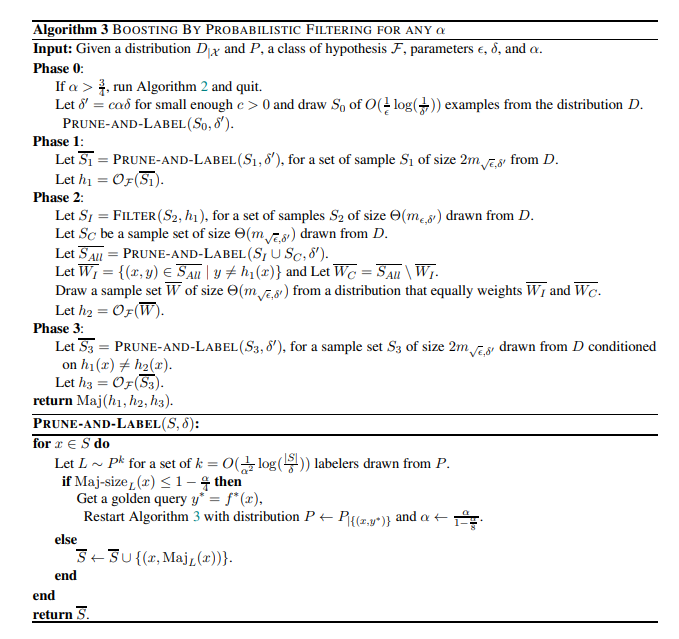
\includegraphics[width=.9\linewidth]{./images/Algo3.png}
\end{center}
\section{5. No perfect lablers exist}
\label{sec:org5ed2d0b}
\begin{itemize}
\item In the case where no perfect labelers exist. We must find a set of good labelers to label our data so that the majority of labelers are correct.
\item This is essentially the agnostic PAC learning framework, and we assume that labelers will be correct with some probability  \(P(x) > \epsilon\) and bad labelers with \(P(x) > 1-4* \epsilon\)
\item Finally we construct the algorithm that where we try and identify a set of labelers who agree with eachother with some high frequency and and since they  should be correct they will form the highest component of a graph
\item Algorithm 4
\end{itemize}
\begin{center}
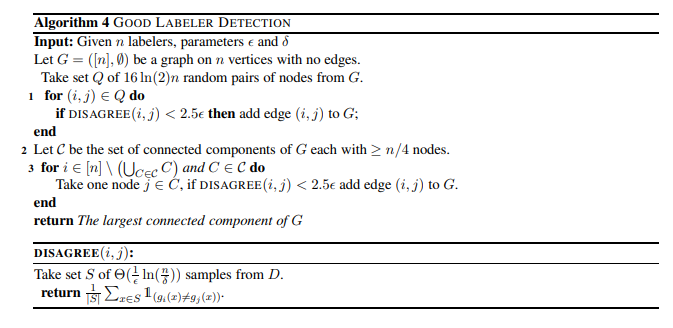
\includegraphics[width=.9\linewidth]{./images/Algo4.png}
\end{center}
\end{document}
